\section{Referencial Teórico}
\label{sec:referencial}

Neste capítulo são apresentadas as tecnologias: robótica autônoma, telemetria, mapeamento, planejamento de trajetória e API, que foram utilizadas para o desenvolvimento do trabalho, com o objetivo de familiarizar o leitor a ter uma leitura mais compreensiva do mesmo.


\subsection{Robótica Autônoma}
A robótica autônoma tem evoluído continuamente, tornando-se cada vez mais relevante no cenário tecnológico atual. A capacidade dos robôs autônomos substituírem humanos em atividades perigosas ou repetitivas justifica os investimentos na área. Competições e projetos educacionais desempenham papel fundamental na formação de profissionais e no estímulo ao interesse pela robótica \cite{RoboAutonomo}.

Alguns dos principais desafios são navegação, planejamento de trajetória, localização e desvio de obstáculos \cite{AMRChallenges}. Os sistemas de navegação de robôs móveis dependem do nível de abstração da representação do ambiente \cite{Mapeamento}. Para determinar com precisão a posição e a orientação do robô móvel, é essencial que o ambiente seja modelado em uma estrutura simples e compreensível.
A parte desafiadora da localização é estimar a posição do robô e a orientação da qual essa informação pode ser obtida de sensores e outros sistemas. Para lidar com o desafio da localização, uma boa técnica deve ser desenvolvida para tratar erros, fatores de interferência, medições incorretas e estimativas imprecisas \cite{Odometria}. Desvio de obstáculos é uma tarefa essencial no campo da robótica, pois é fundamental que o robô alcance seu destino sem ser bloqueado por qualquer obstáculo ou sofrer colisões em seu trajeto \cite{PlanejamentoTrajetoria}. Por esse motivo, algoritmos livres de colisão são um requisito indispensável para robôs móveis autônomos \cite{IntroAR, AMRChallenges}.

Os robôs autônomos têm aplicações variadas: podem atuar desde o campo, monitorando lavouras, até ambientes industriais, seja atuando em processos produtivos como linhas de montagem e gestão logística de estoques em armazéns.

\subsection{ROS}
O Robot Operating System (ROS) é um conjunto de bibliotecas de \textit{software} e ferramentas que auxiliam no desenvolvimento de aplicações robóticas. De \textit{drivers} a algoritmos de ponta, e com poderosas ferramentas para desenvolvedores, o ROS oferece o que você precisa para o seu próximo projeto de robótica. E tudo isso é de código aberto \cite{ROS_Website}.

O ROS vai além de ser apenas um conjunto de bibliotecas, ele funciona como um ecossistema robusto que padroniza a comunicação entre diferentes componentes de software em um robô. Ele oferece um modelo de programação distribuída, onde múltiplos nós (programas executáveis independentes) podem se comunicar enviando e recebendo mensagens através de tópicos. Isso permite que desenvolvedores de diversas áreas colaborem em um mesmo projeto robótico, com cada um focando em um módulo específico (como navegação, percepção ou controle), e o ROS garantindo a integração.

\subsection{Telemetria}
A palavra telemetria é a união de duas palavras gregas. \textit{Tele} significa longe e 
\textit{meter} significa medir. Por isso, telemetria significa realizar medições à distância, ou em local remoto. Os ingredientes essenciais de qualquer sistema de telemetria incluem pelo menos um sensor, uma antena transmissora de baixo ganho, uma antena receptora de alto ganho, um receptor e um mostrador \cite{Telemetria}. 

Teste de veículos foi uma das primeiras aplicações da telemetria. Inicialmente, não tripulados, como mísseis guiados, requeriam telemetria, para que os engenheiros soubessem o que se passava dentro do míssil. Veículos tripulados também requeriam telemetria para medir parâmetros, tais como fadiga da asa, que não eram perceptíveis aos tripulantes 
\cite{Telemetria}.

\subsection{Mapeamento e Planejamento de Trajetória}
A técnica geral de \textit{roadmap} para planejamento de trajetórias consiste em capturar a conectividade do espaço livre do ambiente em uma rede de curvas de uma dimensão, denominada \textit{roadmap}. Uma vez que esta rede tenha sido obtida, ela é vista como um conjunto padrão de caminhos. O planejamento de trajetórias reduz-se então a conectar as posições iniciais e finais do robô ao \textit{roadmap} e buscar neste um caminho entre esses dois pontos, conforme pode ser observado na Figura \ref{fig:roadmap} \cite{PlanejamentoTrajetoria}.

\begin{figure}[h]
    \centering
    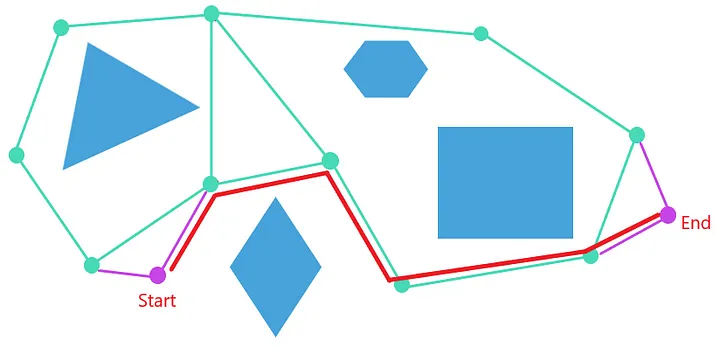
\includegraphics[width=0.45\textwidth]{images/RoadmapRT.png}
    \caption{Gráfico de navegação \textit{roadmap} para encontrar a melhor rota.}
    \label{fig:roadmap}
    % Referência: https://arushi-khokhar.medium.com/probabilistic-roadmap-prm-for-path-planning-in-robotics-d4f4b69475ea
\end{figure}

Quando não há um mapa do ambiente obtido a \textit{priori}, é preciso construir o mapa durante a navegação. Nesse caso, técnicas de localização e mapeamento simultâneo (SLAM) são usadas \cite{SLAM}.

Resolver o problema de SLAM envolve a estimação da trajetória do robô e do mapa do ambiente enquanto o robô se desloca. Ao longo da movimentação do robô em poses sequenciais desconhecidas \( x_{1:t} = x_1, x_2, \ldots, x_t \) em um mapa desconhecido \( m \), são obtidas uma sequência de odometria \( u_{1:t} = u_1, u_2, \ldots, u_t \) e observações do ambiente \( z_{1:t} = z_1, z_2, \ldots, z_t \). O problema SLAM requer a obtenção da distribuição de probabilidades dada pela Equação 1, considerando que \( x_0 \) é a posição inicial do robô \cite{Mapeamento}.

O Cartographer é um sistema de SLAM eficiente que opera em dois níveis: localmente ajusta a pose do robô em submapas usando um \textit{scan matcher} (Ceres), enquanto globalmente refina a localização combinando todos os submapas em um mapa maior \cite{Cartographer, Ceres}. Sua principal vantagem é a flexibilidade, com suporte a múltiplos sensores e resoluções, e a eficiência computacional que permite operação em tempo real \cite{NVIDIA_JetsonOrinNano}.

Existe uma dificuldade intrínseca em conciliar as medições de localização com a posição verdadeira do dispositivo após longos períodos de navegação. O desafio origina-se na imprecisão dos sensores de medidas de odometria (ex: sonares, lasers e câmeras) devido às limitações físicas e imprevisibilidades do sistema \cite{Odometria}.

\subsection{API}
APIs (Interface de Programação de Aplicações) simplificam e aceleram o desenvolvimento de aplicativos e \textit{software}, permitindo que os desenvolvedores integrem dados, serviços e recursos de outros aplicativos, em vez de desenvolvê-los do zero. As APIs também oferecem aos proprietários de aplicativos uma maneira simples e segura de disponibilizar os dados e as funções dos aplicativos para os departamentos da organização. Os proprietários de aplicativos também podem compartilhar ou comercializar dados e funções para parceiros de negócios ou terceiros \cite{IbmAPI}.

As APIs permitem o compartilhamento apenas das informações necessárias, mantendo ocultos outros detalhes internos do sistema, o que auxilia na segurança do sistema. Os servidores ou dispositivos não precisam expor totalmente os dados: as APIs permitem o compartilhamento de pequenos pacotes de dados, relevantes para a solicitação específica \cite{IbmAPI}.

Podem existir vulnerabilidades de segurança devido à implementação da API. Por exemplo, a falha em verificar o tamanho dos \textit{inputs} na sua API pode permitir que um atacante derrube seu servidor ao enviar um \textit{input} extremamente grande que consuma toda a memória disponível - um tipo de ataque de negação de serviço (DoS) \cite{APISecurity}.

ROSBridge é uma especificação de protocolo de rede em camada de aplicação para o ROS (\textit{Robot Operating System}) que enfatiza o modelo cliente/servidor. Especificamente, o ROSBridge permite que clientes publiquem e escrevam mensagens em tópicos e invoquem serviços no ambiente de execução do servidor. O protocolo transporta mensagens formatadas em JSON por meio de \textit{sockets} TCP ou \textit{WebSockets} \cite{ROSBridge}.

No trecho de código \ref{lst:conexao_websocket} a classe roslibpy.ros é instanciada com o IP do dispositivo ROS e também a porta padrão para comunicação WebSocket, e o método client.run() inicia a conexão com o servidor ROS.   

\begin{lstlisting}[caption={Configuração da Conexão WebSocket com ROSBridge},label={lst:conexao_websocket}]
    import roslibpy
    
    # Configura a conexão WebSocket com o ROSBridge
    rosbridge_ws_url = '192.168.137.150'  # IP do dispositivo ROS
    client = roslibpy.Ros(host=rosbridge_ws_url, port=9090)

    # Conecta ao ROS
    client.run()
\end{lstlisting}
    
\subsection{Articulação das Tecnologias}
As tecnologias apresentadas neste referencial teórico articulam-se de forma coerente e complementar na solução desenvolvida. A robótica autônoma fornece a base conceitual para o sistema, enquanto as técnicas de telemetria e os protocolos de comunicação (ROSBridge) garantem a troca eficiente de dados entre os componentes. O SLAM e os algoritmos de planejamento de trajetória permitem a navegação autônoma, sendo acessíveis ao usuário através da interface desenvolvida com \textit{frameworks} modernos. As APIs, por sua vez, atuam como elemento integrador, possibilitando a comunicação segura entre a aplicação e o sistema robótico. Esta sinergia tecnológica resulta em uma plataforma completa que aborda desde a percepção ambiental até a interação com o usuário final, cumprindo os objetivos propostos de forma integrada e eficiente.